%% \chapter[htoc-titlei][hhead-titlei]{htitlei}
%% -----------------------------------------------------------------------------
\chapter[Theoretical Framework][Theoretical Framework]{Theoretical Framework} \label{ch:theory}

This chapter outlines the theoretical groundwork for the rest of the thesis.
An overview of the Standard Model of particle physics (SM) is given in Section~\ref{sec:theory_sm}, followed by the electroweak symmetry breaking mechanism involving the Higgs boson in Section~\ref{sec:theory_higgs}.
Finally, Section~\ref{sec:theory_vbs} will go into detail on the interests of electroweak vector boson scattering (VBS).

\section{Introduction to the Standard Model} \label{sec:theory_sm}
%Modern particle physics is generally interpreted in terms of the Standard Model (SM).
%This is a quantum field theory which encapsulates our understanding of the electromagnetic, weak, and strong interactions...

The Standard Model of particle physics serves as a mathematical description of the fundamental particles of the universe and their interactions.
It has been developed over the course of the past century, incorporating both predictions from theory and results from experiments.
All in all, the SM has proven remarkably successful in accurately describing particle interactions seen in experiments.

The SM is a quantum field theory (QFT)~\cite{1995.Weinberg, 1995.Peskin} in which the fundamental particles are represented as excited states of their corresponding fields.
The spin-$\frac{1}{2}$ fermionic fields give rise to the quarks and leptons comprising ordinary matter, the spin-1 fields correspond to the electroweak bosons and the gluon which mediate the electroweak and strong forces, respectively, and finally the scalar Higgs field is responsible for electroweak symmetry breaking.
The excitations and interactions of the fields are governed by the SM Lagrangian, which is invariant under local transformations of the group $\gtsu{3}\times\gtsu{2}\times\gtu{1}$.
\TODO{need more detail/refinement here}

The first quantum field theory to be developed was quantum electrodynamics (QED)~\cite{1950.Feynman.QED}, which describes the electromagnetic interaction.
The theory predicts the existence of a $\gtu{1}$ gauge field that interacts with the electrically charged fermions.
This field corresponds to the photon.
A key aspect of QED is that it is perturbative.
The coupling constant $\alpha = e^2/4\pi$ is small, where $e$ is electrical charge of the field, allowing for the use of perturbation theory in calculations.
In this case, calculations can be written as a power series in $\alpha$, where successive higher order terms contribute less to the final result.
%\TODO{renormalizability here?}

The strong interaction---the theory of quarks and gluons---has also been described using QFT as quantum chromodynamics (QCD).
%QCD is the theory of quarks and the associated strong force-carrier the gluon.
The symmetry group for QCD is $\gtsu{3}$, and its eight generators correspond to the eight differently charged, massless gluons~\cite{1965.Han-Nambu.Propose-color}.
Unlike in QED, which has positive and negative charges, the strong force has three ``colors''.
Color charge combined with the non-Abelian nature of $SU(3)$, which allows the gluons to interact with each other, result in the most well-known property of QCD: color confinement.
In order to increase the separation between two color-charged quarks, the amount of energy required increases until it becomes energetically favorable to pair-produce a new quark-antiquark pair, which then bind to the original quarks.
The end result of this is that only color-neutral objects exist in isolation. % and it is responsible for the hadronic jets in experiments.
What this means for the strong coupling constant $\alpha_s$ is that its value at the low energies where confinement occurs is large, on the order of $\alpha_s\sim 1$.
The consequense of this is that perturbation theory cannot be used to accurately approximate interactions.
While this appears at first to be a critical problem for predictions, fortunately it turns out that $\alpha_s$ ``runs'', or decreases in magnitude at higher energy~\cite{1973.asymptotically-free-i, 1974.asymptotically-free-ii}.
This so-called ``asymptotic freedom'' allows QCD to be calcualted perturbatively~\cite{1973.strong-perturbation} at energies accessible by collider experiments including the LHC.
%A second important property of the QCD is that, unlike in QED, the coupling constant $\alpha_s$ is large at low energies where confinement occurs, and thus it cannot be described accurately using perturbation theory.
%Fortunately, $\alpha_s$ ``runs'', or decreases at higher energy scales~\cite{1973.asymptotically-free-i, 1974.asymptotically-free-ii}; this allows QCD to be calculated perturbatively~\cite{1973.strong-perturbation} at energies accessible by collider experiments including the LHC.

The last gauge field corresponds to the weak interaction.
Ultimately, the weak $\gtsu{2}$ and the electromagnetic $\gtu{1}$ mix to form the $\gtsu{2}\times\gtu{1}$ \emph{electroweak} (EWK) interaction~\cite{1959.Salam.electroweak, 1959.Glashow.vector-mesons}.
A more detailed description of the mixing will be discussed in conjunction with electroweak symmetry breaking (EWSB) in Section~\ref{sec:theory_higgs}; however, a summary of the resulting EWK interaction is presented here, at the risk of some repeated information to follow.
There are three weak isospin bosons arising from the $\gtsu{2}$ group ($W_{\mu}^1$, $W_{\mu}^2$, and $W_{\mu}^3$) and one weak hypercharge boson from the $\gtu{1}$ group ($B_{\mu}$).
The $W_3$ and $B$ bosons mix according to the weak mixing angle $\theta_W$ to form the $Z$ boson and the photon according to:
\begin{equation}
  \begin{pmatrix}
  \gamma\\
  Z
  \end{pmatrix}
  = 
  \begin{pmatrix}
  \cos{\theta_W} & \sin{\theta_W} \\
  -\sin{\theta_W} & \cos{\theta_W}
  \end{pmatrix}
  \begin{pmatrix}
  B_{\mu} \\
  W_{\mu}^3
  \end{pmatrix}
  \label{eq:weak_mixing}
\end{equation}
The value of $\theta_W$ is not predicted by the SM; it is one example of an experimental input to the theory, measured to be $\sin^2{\theta_W} = 0.23153\pm0.00016$~\cite{2006.weak-mixing}.
The charged $W^{\pm}$ bosons are a mixture of the remaining $W_{\mu}^1$ and $W_{\mu}^2$ bosons:
\begin{equation}
  W^{\pm} = \frac{1}{\sqrt{2}}(W_{\mu}^1 \mp iW_{\mu}^2)
  \label{eq:w_mixing}
\end{equation}
Unlike the photon (and the gluon of QCD), the $W^\pm$ and $Z$ bosons are massive.
This means that even though $\gtsu{2}$ is non-Abelian, the range of interaction is short and confinement does not occur.
Lastly, the EWK interaction is chiral, only coupling to the left-handed component of the fermion fields

One final field remains within the SM: the scalar Higgs field.
It was originally proposed in the 1960's to explain the masses of the $W^{\pm}$ and $Z$ bosons~\cite{1964.Englert.symmetry_breaking, 1964.Higgs.Broken_Symmetries_1, 1964.Higgs.Broken_Symmetries_2} and is the mechanism for the EWSB process.
The particle associated with the field is a massive scalar boson, which was at last discovered by ATLAS and CMS in 2012~\cite{HIGG-2012-27, CMS-HIG-12-028} with a mass of $125\gev$.


%\subsection{Electroweak mixing}\label{theory:ewk_mixing}
%\begin{itemize}
%  \item intro: theory+experimental motivation, four forces, blah
%  \item paragraph about what QFT is
%  \item Gauge invariance, renormalizibility of lagrangian (useful for the WW stuff later)
%  \item Electromagnetism - QED, $\alpha$, perturbation theory
%  \item Electroweak - mixing with EM, W/Z/$\gamma$, self-interacting is important for T/QGC, left handed
%  \item Strong - confinement, asymptotic freedom
%  \item Higgs - introduce it here w/ separate section after, source of mass for fermion/boson, discovery reference
%\end{itemize}


\section{Electroweak symmetry breaking and the Higgs boson} \label{sec:theory_higgs}
%When the theory of the electroweak interaction was first developed \cite{1959.Glashow.vector-mesons, 1959.Salam.electroweak},
%the $W$ and $Z$ bosons were predicted to be massless (a typical mass term in the Lagrangian would violate the SU(2) symmetry).
%However, these were experimentally observed to have masses...

The results of electroweak mixing and the implications of the Higgs field have been introduced in the previous section.
If the EWK theory were an unbroken symmetry, the associated $W^{\pm}$ and $Z$ bosons would be massless; however, when first observed experimentally~\cite{1983.w-boson, 1983.z-boson}, they were found to be quite heavy; currently, their masses are known to be approximately $80\gev$ and $91\gev$, respectively~\cite{2014.pdg}.
The following presents the Higgs mechanism, including how it ``spontaneously breaks'' the EWK symmetry, resulting in the massive $W^\pm$ and $Z$ bosons and the massless photon.

Beginning by writing the Higgs field as a complex scalar doublet %$\phi$
\begin{equation}
  \phi = 
  \begin{pmatrix}
    \phi^{+} \\
    \phi^{0}
  \end{pmatrix}
  = \sqrt{\frac{1}{2}}
  \begin{pmatrix}
    \phi_1 + i\phi_2 \\
    \phi_3 + i\phi_4
  \end{pmatrix}\,,
  \label{eq:complex_scalar_doublet}
\end{equation}
a simple Lagrangian $\mathcal{L}$ can be written as
\begin{equation}
  \mathcal{L} = (\mathcal{D}_\mu\phi)^\dagger (\mathcal{D}^\mu\phi) - \mu^2\phi^{\dagger}\phi-\lambda (\phi^{\dagger}\phi)^2\,,
  \label{eq:complex_scalar_lagrangian}
\end{equation}
where $\lambda > 0$ and $\mu^2$ are constants (the sign of $\mu^2$ will be addressed shortly).
$\mathcal{D}_{\mu}$ is the covariant derivative defined such that $\mathcal{L}$ is invariant under a local $\gtsu{2}\times\gtu{1}$ gauge transformation:
\begin{equation}
  \mathcal{D}_{\mu}\phi = \bigg(\partial_{\mu} + \frac{ig}{2}\tau_a W_{\mu}^a + \frac{ig'}{2}B_{\mu}\bigg)\phi\,.
  \label{eq:covariant_deriv}
\end{equation}
Here, $W_{\mu}^a$ ($a=1,2,3$) are the $\gtsu{2}$ fields with generators $\tau_a$ and coupling constant $g$, and $B_{\mu}$ is the $\gtu{1}$ field with coupling constant $g'$.

Isolating the Lagrangian's potential term,
\begin{equation}
  V(\phi) = \mu^2\phi^{\dagger}\phi+\lambda(\phi^{\dagger}\phi)^2\,,
  \label{eq:higgs_potential}
\end{equation}
a choice must be made on the sign of $\mu^2$.
The case of interest is when $\mu^2 < 0$, which results in the so-called ``Mexican hat potential'' shown in Figure~\ref{fig:mexican_hat}.
The potential is minimized along the collection of points
\begin{equation}
  \phi^{\dagger}\phi = \frac{1}{2}\big(\phi_1^2 + \phi_2^2 + \phi_3^2 + \phi_4^2\big) = -\frac{\mu^2}{2\lambda}\,.
  \label{eq:higgs_minimum}
\end{equation}
This means that the minimum of the potential is not at $\phi = 0$ (as it would be in the case where $\mu^2 > 0$), but rather at a value
\begin{equation}
  v \equiv \sqrt{-\frac{\mu^2}{\lambda}}\,.
  \label{eq:higgs_minimum_value}
\end{equation}
With no loss of generality due to the $\gtsu{2}$ symmetry, $\phi_1 = \phi_2 = \phi_4 = 0$ can be imposed on Equation~\ref{eq:higgs_minimum}, leaving $\phi_3^2 = v^2$.
Finally, the \emph{vacuum expectation value} (VEV) of the field can be written:
\begin{equation}
  \langle\phi\rangle = \sqrt{\frac{1}{2}}
  \begin{pmatrix}
  0 \\ v
  \end{pmatrix}\,.
  \label{eq:vev}
\end{equation}

\begin{figure}[htbp]
  \centering
  \includegraphics[width=.48\textwidth]{figs/theory/higgspotential_greater0}
  \includegraphics[width=.48\textwidth]{figs/theory/higgspotential}
  \caption{An illustration of the potential term $V(\phi)$ in Equation~\ref{eq:higgs_potential} for the cases where $\mu^2>0$ (left) and $\mu^2<0$ (right).  The right-hand plot shows the Higgs potential, or ``Mexican hat potential'', with the minimum at $|\phi| = \sqrt{-\frac{\mu^2}{\lambda}}$ rather than at $|\phi| = 0$ as in the left-hand plot.}
  \label{fig:mexican_hat}
\end{figure}

The VEV can be substituted back into the original Lagrangian of Equation~\ref{eq:complex_scalar_lagrangian}, and, following quite a bit of math~\cite{1984.halzen-martin}, a collection of mass terms can be identified:
\begin{equation}
  \mathcal{L} \subset \mathcal{L}_M \equiv \frac{1}{8}v^{2}g^{2}\bigg[\big(W_{\mu}^1\big)^2 + \big(W_{\mu}^2\big)^2\bigg] + \frac{1}{8}v^2\bigg[g^{2}\big(W_{\mu}^3\big)^2 - 2gg'W_{\mu}^{3}B^{\mu} + g'^{2}\big(B_{\mu}\big)^{2}\bigg]\,.
  \label{eq:higgs_mass_1}
\end{equation}
Focusing on the first term for the moment, if Equation~\ref{eq:w_mixing} for the physical $W^\pm$ bosons is substituted in, the mass term becomes
\begin{equation}
  M_W^{2}W^{+}W^{-} = \bigg(\frac{1}{2}vg\bigg)^{2}W^{+}W^{-}\,,
\end{equation}
which then simplifies to
\begin{equation}
  M_W = \frac{1}{2}vg\,.
\end{equation}
With a bit of clever forward-thinking, the second term of Equation~\ref{eq:higgs_mass_1} can be rewritten as
\begin{equation}
  \frac{1}{8}v^{2}\bigg[gW_{\mu}^{3} - g'B_{\mu}\bigg]^2 + 0\bigg[g'W_{\mu}^{3} - gB_{\mu}\bigg]^2 =  \frac{1}{2}M_{Z}^{2}Z_{\mu}^{2} + \frac{1}{2}M_{A}^{2}A_{\mu}^{2}\,,
  \label{eq:higgs_mass_2}
\end{equation}
where $Z_{\mu}^{2}$ and $A_{\mu}^2$ represent the physical $Z$ boson and photon, respectively:
\begin{equation}
 Z_{\mu} = \frac{gW_{\mu}^{3} - g'B_{\mu}}{\sqrt{g^2+g'^2}}
  \label{eq:higgs_z}
\end{equation}
\begin{equation}
  A_{\mu} = \frac{g'W_{\mu}^{3} - gB_{\mu}}{\sqrt{g^2+g'^2}}\,.
  \label{eq:higgs_a}
\end{equation}
From this, it can be seen that the photon is massless ($M_A = 0$ in Equation~\ref{eq:higgs_mass_2}), and the mass of the $Z$ boson is identified as
\begin{equation}
  M_Z = \frac{1}{2}v\sqrt{g^2+g'^2}\,.
\end{equation}

Lastly, the Higgs field can couple directly to the fermions.
Taking the electron as an example, an additional Lagrangian term can be written:
\begin{equation}
\mathcal{L}_e = -G_e \big[\bar{e}_{L}\phi e_R+\bar{e}_R\phi^{\dagger}e_L\big]\,,
\end{equation}
where $e_L$ and $e_R$ are the left-handed doublet and right-handed singlet, respectively, and $\phi$ is as in Equation~\ref{eq:complex_scalar_doublet}.
The symmetry can be spontaneously broken by a perturbation about the VEV of the form
\begin{equation}
  \phi = \sqrt{\frac{1}{2}}
  \begin{pmatrix}
  0 \\ v+h(x)
  \end{pmatrix}\,.
\end{equation}
$\mathcal{L}_e$ then becomes
\begin{equation}
  \begin{aligned}
    \mathcal{L}_e &= -\frac{G_e}{\sqrt{2}}v\big(\bar{e}_{L}e_{R}+\bar{e}_{R}e_{L}\big) - \frac{G_e}{\sqrt{2}}\big(\bar{e}_{L}e_{R}+\bar{e}_{R}e_{L}\big)h \\
                  &= -m_e\bar{e}e-\frac{m_e}{v}\bar{e}eh\,,
  \end{aligned}
\end{equation}
which gives a value for the electron mass of $m_e = \frac{G_{e}v}{\sqrt{2}}$.
From the second term above, it can be seen that the strength of the Higgs coupling to the electron is proportional to the mass of the electron.
The rest of the fermion couplings follow from this example.

What is accomplished here is quite remarkable.
The weak and electromagnetic interactions have been unified into a single $\gtsu{2}\times\gtu{1}$ interaction, and the physical bosons observed in nature arise as mixtures of the four gauge fields.
Three of the four degrees of freedom in the scalar field $\phi$ of Equation~\ref{eq:complex_scalar_doublet}, are absorbed (or ``eaten'') by the $W^{\pm}$ and $Z$ bosons, giving them a longitudinal polarization mode corresponding to a massive particle, and the fourth generates the Higgs boson.
This process is summarized in Figure~\ref{fig:higgs_dof}.
Additionally, it is shown that the Higgs couples to fermions in proportion to their mass.
From experimental measurements, the value of the VEV has been determined to be $v\approx 246\gev$~\cite{2014.pdg}.
However, it should be noted that the theory does not predict the mass of the Higgs boson or of the fermions; these must all be determined from experiment.

\begin{figure}[htbp]
  \centering
  \includegraphics[width=.65\textwidth]{figs/theory/higgs_mechanism_dof}
  \caption{A graphical representation of the EWSB mechanism involving the $\gtsu{2}\times\gtu{1}$ bosons and the Higgs field.  The $W^\pm$ and $Z$ bosons each obtain mass by eating a degree of freedom (dof) from the Higgs field, and in the process gain a longitudinal polarization mode, while the photon stays massless (with two dof) and the SM Higgs boson $h$ remains.}
  \label{fig:higgs_dof}
\end{figure}


%\section{Diboson physics}\label{sec:theory_diboson}
%%TGC: WWg WWZ
%QGC: WWZg WWgg WWWW WWZZ
Processes involving two final state gauge bosons are of particular interest for testing the predictive power of the SM.
Due to the non-Abelian nature of the EWK interaction, the corresponding gauge bosons are allowed to self-interact.
This results in triple and quartic couplings of gauge bosons (TGCs and QGCs, respectively).
The SM allowed TGCs are the $WW\gamma$ and $WWZ$ vertices, and the QGCs predicted by the model include $WWZ\gamma$, $WW\gamma\gamma$, $WWZZ$, and $WWWW$.
These vertices are accessible via a number of production modes at hadron colliders, including vector boson fusion and scattering (VBF and VBS, as in Figure~\ref{fig:theory_vbf_vbs}).
The LHC in particular has provided the first opportunity to observe some of these vertices, such as the $WW\gamma\gamma$ QGC via the $W\gamma\gamma$ final state~\cite{2015.wgg}, or the $WWWW$ QGC via same-sign $W^{\pm}W^{\pm}$ production~\cite{2014.ssww-8tev-atlas}.
Precise measurements of these processes can be compared to the theoretical predictions, and deviations can point to deficiencies in the prediction, such as needing an additional order in $\alpha_s$ in the calculation, or even hints at new physics, like anomalous gauge couplings\footnote{In the SM, the TGCs and QGCs are fixed by the electromagnetic coupling constant $\alpha$ and the electroweak mixing angle $\theta_W$.  In many Beyond the Standard Model scenarios, these couplings are modified by additional contributions.}~\cite{2017.anomalous-tgc-lhc}.

\begin{figure}[htbp]
  \centering
  \includegraphics[height=.13\textheight]{figs/theory/vbf}\hspace{20pt}
  \includegraphics[height=.13\textheight]{figs/theory/vbs}
  \caption{Vector boson fusion involving triple gauge couplings (left) and vector boson scattering involving a quartic gauge coupling (right).}
  \label{fig:theory_vbf_vbs}
\end{figure}

Diboson interactions also make up one of the most sensitive tests of EWSB.
Aside from the top quark, the EWK bosons have the strongest coupling to the Higgs mechanism, as there are several production diagrams involving the exchange of a Higgs boson, including those in Figure~\ref{fig:theory_higgs}.
In this instance, VBS processes are particularly important as the Higgs unitarizes the scattering amplitude~\cite{1977.ben-lee-weak-interactions-physrevd} (this particular aspect will be explored in more detail in the context of same-sign $W^{\pm}W^{\pm}$ scattering in Section~\ref{ssww13tev:vbs_theory}).
Since the Higgs boson has only recently been discovered, it has not yet been extensively tested, and there could still be deviations in the EWSB mechanism that may manifest in the VBF and VBS measurements~\cite{2017.multiboson-at-lhc}.

\begin{figure}[htbp]
  \centering
  \includegraphics[width=.3\textwidth]{figs/theory/higgs_s}\hspace{20pt}
  \includegraphics[width=.3\textwidth]{figs/theory/higgs_t}
  \caption{Diboson diagrams involving the $s$-channel (left) and $t$-channel (right) exchanges of a Higgs boson.}
  \label{fig:theory_higgs}
\end{figure}

%An alternative scenario involves anomalous couplings~\cite{2017.anomalous-tgc-lhc}.
%In the SM, the TGCs and QGCs are fixed by the electromagnetic coupling constant $\alpha$ and the electroweak mixing angle $\theta_W$.
%However, in many Beyond the Standard Model (BSM) scenarios, these couplings are modified by additional BSM contributions.
%In this case, the SM Lagrangian is considered to be one component of an overall effective Lagrangian


\section{Electroweak vector boson scattering}\label{sec:theory_vbs}
Due to the non-Abelian nature of the EWK interaction, the associated gauge bosons are allowed to self-interact.
This results in triple and quartic couplings of gauge bosons (TGCs and QGCs, respectively).
The SM allowed TGCs are the $WW\gamma$ and $WWZ$ vertices, which can be measured experimentally via diboson production or through vector boson fusion (VBF).
The QGCs predicted by the SM are $WWZ\gamma$, $WW\gamma\gamma$, $WWZZ$, and $WWWW$, and these vertices are accessible via triboson production or vector boson scattering (VBS)\footnote{Vector boson fusion and scattering typically refer to the $s$-channel and $t$-channel exchanges of a vector boson, respectively; however, often both are used interchangeably to describe the $VV\rightarrow VV$ process.  Therefore, for the remainder of this thesis, \emph{vector boson scattering} will refer to both the VBF and VBS production mechanisms.}~\cite{2017.multiboson-at-lhc}.
VBS processes are defined by a $VV\rightarrow VV$ signature, where $V$ represents one of the EWK gauge bosons ($W^{\pm}$, $Z$, or $\gamma$), as shown in Figure~\ref{fig:theory_generic_vbs}.
The actual interaction between the incoming and outgoing vector bosons can be mediated by the exchange of a virtual $V$, directly via a QGC (both are shown in Figure~\ref{fig:theory_vbs_ewk}), or by the exchange of a Higgs boson (as in Figure~\ref{fig:theory_vbs_higgs}).

\begin{figure}[htbp]
  \centering
  \includegraphics[width=.4\textwidth]{figs/theory/generic_vbs}
  \caption{Feynman diagram of a generic VBS process.  The gray circle represents any interaction with two incoming and two outgoing vector bosons, including any of the diagrams shown in Figures~\ref{fig:theory_vbs_ewk} and \ref{fig:theory_vbs_higgs}.}
  \label{fig:theory_generic_vbs}
\end{figure}

\begin{figure}[htbp]
  \centering
  \includegraphics[height=.125\textheight]{figs/theory/vbs_ewk}
  \caption{Leading order $VV\rightarrow VV$ Feynman diagrams involving EWK bosons. From left to right: $s$-channel, $t$-channel, $u$-channel, and the quartic gauge coupling.}
  \label{fig:theory_vbs_ewk}
\end{figure}
\begin{figure}[htbp]
  \centering
  \includegraphics[height=.125\textheight]{figs/theory/vbs_higgs}
  \caption{Leading order $VV\rightarrow VV$ Feynman diagrams involving the exchange of a Higgs boson. From left to right: $s$-channel, $t$-channel, and $u$-channel.}
  \label{fig:theory_vbs_higgs}
\end{figure}

As detailed in the previous section, the Higgs mechanism produces three Goldstone bosons and a Higgs boson.
The Goldstone bosons are then ``eaten'' by the physical gauge bosons, giving them mass and consequently a longitudinal polarization\footnote{A massless spin-1 boson can have one of two transverse polarization states, while a massive spin-1 boson can also be longitudinally polarized.  As a result, only the massive $W^{\pm}$ and $Z$ bosons, and not the massless photon, are sensitive to EWSB.}.
In fact, according to the Electroweak Equivalence Theorem, the high-energy interactions of longitudinal gauge bosons can be accurately described by the Goldstone bosons of the EWSB mechanism~\cite{1997.ewk-equivalence}.
Thus, the scattering of the massive gauge bosons is inextricably linked to EWSB.

It turns out that without a light SM Higgs boson, the scattering amplitude of longitudinally polarized vector bosons grows with center-of-mass energy and ultimately violates unitarity above $\sqrt{s}\approx 1.2\tev$~\cite{1977.ben-lee-weak-interactions, 2009.strong-gauge-boson-scattering}.
Writing down the equations for the transverse and longitudinal polarization vectors for a gauge boson of mass $M_V$~\cite{1990.strong-ww-scattering}:
\begin{equation}
  \epsilon^{\mu}_{\pm} = \frac{1}{\sqrt{2}}(0,0,\pm i, 0)
\end{equation}
\begin{equation}
  \begin{aligned}
    \epsilon^{\mu}_L &= \frac{1}{M_V}(|\vec{p}|, 0, 0, E)\\
                    &= \frac{p^{\mu}}{M_V}+v^{\mu}
  \end{aligned}
  \label{eq:longitudinal_polarization}
\end{equation}
where $v^{\mu}$ is of the order $M_V/E$ and becomes small in the high energy limit, it can be seen that $\epsilon^{\mu}_{L}$ grows with the momentum of the boson $p^{\mu}$.
Therefore, the dominant contribution to the VBS process at high energy comes from the longitudinally polarized gauge bosons~\cite{2012.vbs-thesis-oord}.

% reference diagrams above, then do the matrix element thing (StrongGaugeBosonScatteringTheory.pdf sec 1.1), and cite the figure below
The high-energy behavior of longitudinally polarized vector boson scattering can be explored in the case of opposite-sign $W^{+}W^{-}\rightarrow W^{+}W^{-}$ scattering.
In the high-energy limit ($s \gg M_W^2, M_H^2$), the amplitude of $W^{+}W^{-}$ scattering without considering the Higgs contributions (the appropriate diagrams from Figure~\ref{fig:theory_vbs_ewk}) can be written as~\cite{2009.strong-gauge-boson-scattering}:
\begin{equation}
  \mathcal{M}_{\textrm{gauge}} = -\frac{g^2}{4M_W^2}u+\mathcal{O}\Bigg(\bigg[\frac{E}{M_W}\bigg]^0\Bigg)
  \label{eq:theory_longitudinal_m_gauge}
\end{equation}
where $g$ is the EWK coupling and $u$ is one of the Mandelstam variables (the others being $s$ and $t$).
The $\mathcal{O}(E^4)$ terms cancel out between the TGC and QGC diagrams~\cite{2012.vbs-thesis-oord}.
What is left is an amplitude proportional to $E^2$ that diverges as $E/M_W\rightarrow\infty$.
However, the amplitude from the diagrams involving the Higgs boson (the relevant diagrams from Figure~\ref{fig:theory_vbs_higgs}) is:
\begin{equation}
  \mathcal{M}_{\textrm{Higgs}} = -\frac{g^2}{4M_W^2}\bigg[\frac{(s-M_W^2)^2}{s-m_H^2}+\frac{(t-M_W^2)^2}{t-M_H^2}\bigg]
\end{equation}
which, in the high-energy limit, reduces to:
\begin{equation}
  \mathcal{M}_{\textrm{Higgs}} = \frac{g^2}{4M_W^2}u+\mathcal{O}\Bigg(\bigg[\frac{E}{M_W}\bigg]^0\Bigg)
  \label{eq:theory_longitudinal_m_higgs}
\end{equation}
Adding the two equations together cancels out the $E^2$ term and leaves only terms constant in energy.
Therefore, with a SM Higgs, the scattering amplitude for longitudinally polarized $W$ bosons no longer diverges.
Plots of the cross section of several $VV\rightarrow VV$ scattering processes are shown in Figure~\ref{fig:theory_vbs_xsec_higgs} with and without a SM Higgs boson.

\begin{figure}[htbp]
  \centering
  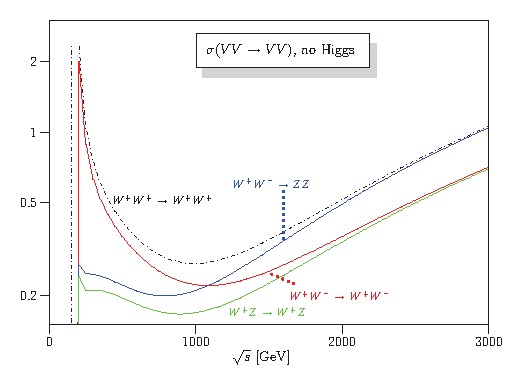
\includegraphics[height=.25\textheight]{figs/ssww_13tev/introduction/vbs_xsec_nohiggs}
  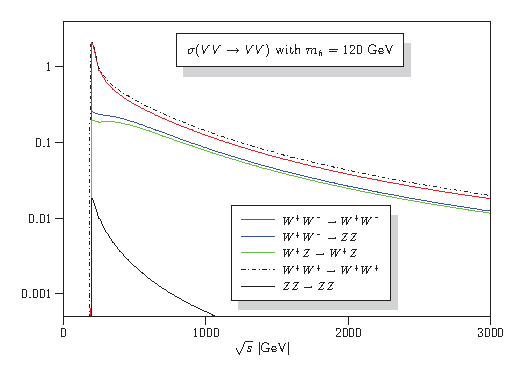
\includegraphics[height=.25\textheight]{figs/ssww_13tev/introduction/vbs_xsec_higgs120}
 
  \caption[Cross sections in nanobarns for five different longitudinally polarized VBS processes as a function of center of mass energy $\sqrt{s}$.  Without a Higgs boson (left), the cross sections grow unbounded with $\sqrt{s}$. With a $120\gev$ Higgs boson (right), the cross sections no longer diverge.]{Cross sections in nanobarns for five different longitudinally polarized VBS processes as a function of center of mass energy $\sqrt{s}$.  Without a Higgs boson (left), the cross sections grow unbounded with $\sqrt{s}$. With a $120\gev$ Higgs boson (right), the cross sections no longer diverge.  Plots taken from~\cite{2008.vbs-resonances-unitarity}.}
  \label{fig:theory_vbs_xsec_higgs}
\end{figure}

